\section{Numerical experiments. }

In this section, we compare the theoretical results, to the numerical results obtained with \texttt{Basilisk} introduced in \ref{chap:DNS}. 
We recall that we are working with a set of simulations covering the parameter ranges displayed in \ref{tab:simulations_recall}. 
\begin{table}[h!]
    \centering
    \caption{Dimensionless parameter range investigated in this work.}
    \begin{tabular}{|ccccccc|ccc|}
        \hline
        \multicolumn{7}{|c}{Primary parameters} & \multicolumn{3}{||c|}{Secondary parameters}\\ \hline
        \multicolumn{1}{|c|}{$Ga$}                               & \multicolumn{1}{c|}{$Bo$}                   & \multicolumn{1}{c|}{$\phi$} & \multicolumn{1}{c|}{$\lambda$}                    & \multicolumn{1}{c|}{$\zeta$}                & \multicolumn{1}{c|}{$N_b$} & $t^*_\text{end}$ & \multicolumn{1}{||c|}{$\mathcal{L}/d$} & \multicolumn{1}{c|}{$Re$}  & $We$   \\ \hline
        \multicolumn{1}{|c|}{\multirow{4}{*}{$5\rightarrow 80$}} & \multicolumn{1}{c|}{\multirow{4}{*}{$0.5$}} & \multicolumn{1}{c|}{$1\%$}  & \multicolumn{1}{c|}{\multirow{4}{*}{$10$ \& $1$}} & \multicolumn{1}{c|}{\multirow{4}{*}{$0.9$}} & \multicolumn{1}{c|}{$160$} & $400$           & \multicolumn{1}{||c|}{$20$}            & \multicolumn{1}{c|}{$1.1\to 110$} & {$0.03\to 0.95$} \\ 
        \multicolumn{1}{|c|}{}                                   & \multicolumn{1}{c|}{}                       & \multicolumn{1}{c|}{$5\%$}  & \multicolumn{1}{c|}{}                             & \multicolumn{1}{c|}{}                       & \multicolumn{1}{c|}{$800$} & $400$           & \multicolumn{1}{||c|}{$20$}            & \multicolumn{1}{c|}{$0.8\to 92$} &  {$0.02\to 0.67$}\\ 
        \multicolumn{1}{|c|}{}                                   & \multicolumn{1}{c|}{}                       & \multicolumn{1}{c|}{$10\%$} & \multicolumn{1}{c|}{}                             & \multicolumn{1}{c|}{}                       & \multicolumn{1}{c|}{$200$} & $1000$           & \multicolumn{1}{||c|}{$10$}            & \multicolumn{1}{c|}{$0.64\to 77$}&  {$0.01\to 0.47$}\\ 
        \multicolumn{1}{|c|}{}                                   & \multicolumn{1}{c|}{}                       & \multicolumn{1}{c|}{$20\%$} & \multicolumn{1}{c|}{}                             & \multicolumn{1}{c|}{}                       & \multicolumn{1}{c|}{$400$} & $1000$           & \multicolumn{1}{||c|}{$10$}            & \multicolumn{1}{c|}{$0.43\to 62$}&  {$9\cdot 10^{-3}\to 0.31$}\\ \hline
        \end{tabular}
    \label{tab:simulations_recall}
\end{table}
In the first step, we will make use of the simulation results at $Ga = 5$ which is considered to be comparable to the Stokes regime used for the theory. 
However, note that at $Ga = 5$, $Re \approx 1$ consequently inertial effects are already present. 
Nevertheless, due to numerical constraints lower \textit{Reynolds} numbers could not be reached. 

The two main results that we are seeking to validate are, the disturbance fields expression \eqref{eq:v_nst_solution_adim} and the \textit{Reynolds} stress closure tensor, \eqref{eq:functional_form_avg}. 
Consequently, in the first part of this section, we focus on the comparison of $\textbf{v}_f^\text{nst}$ obtained with the DNS to the solution given by \ref{eq:v_nst_solution_adim}.
Then, we compare the numerical value of $\avg{\chi_f \textbf{u}_f'\textbf{u}_f'}$ with the prediction of \ref{eq:functional_form_avg}. 
Finally, our goal will be to extend \ref{eq:functional_form_avg} to non-negligible inertial effect and volume fraction effects, i.e. to higher $Re$ and $\phi$. 

\subsection{Nearest neighbors conditionally averaged disturbance velocity}

To reconstruct $\textbf{v}_f^\text{nst}$ with the DNS we must discretize \ref{eq:def_f_nst}. 
We proceed as follows: 
(1) We consider all simulations time steps and locations in the mesh as an independent configuration $\FF$.
This assumption holds since the system is homogeneous and statistically steady in time.  
Thus, we consider that the field $\textbf{u}_f^0[\textbf{x},\FF,t]$ is given by the field $\textbf{u}[c,t]$, where $c$ is the label of a given cell in the mesh and $t$ the time step of the simulation. 
Here, it must be understood that $\FF$ corresponds to all different combinations of $c$ and $t$. 
(2) Finally, we discretize the distance vector $\textbf{r}$ from a point in the mesh to the center of mass of the nearest neighbor, in $n^{th}$ intervals, with the location of the center of the $k^{th}$ interval denoted by $\textbf{r}_k$, where $\textbf{r}_k = 1,\ldots,n$. 
Under these hypotheses, the \textit{nearest neighbors conditionally averaged} velocity fields, $\textbf{u}_f^\text{nst}$, can be obtained numerically as, 
\begin{equation}
    \textbf{u}_f^\text{nst}(\textbf{r}_k)
    = 
    \frac{1}{E_k}
    \sum_{\FF_k}^{E_k}
    \sum_i^N
    \textbf{u}[c,t] h_i[c,t],
    \label{eq:vnst_DNS}
\end{equation}
where $E_k$ corresponds to the total number of events and $N$ to the total number of particles in the flow.
$h_i[c,t]$ corresponds to the function $h_i[\textbf{x},t,\FF]$  (see \ref{eq:h_i_def}), evaluated at time step $t$ and at the center of cell $c$. 
Thus, $h_i[c,t] = 1$ when the $i^{th}$ droplet is the nearest neighbor to the location of the cell center $c$. 
$h_i[c,t]$ is a function of the droplet's center of mass positions, which are obtained using the same approach as in the previous chapters.
Then, to recover $\textbf{v}_f^\text{nst}/U$ from $\textbf{u}_f^\text{nst}$, we simply measure the mean relative phase velocity $U$ within the DNS, and use the formula: $\textbf{v}_f^\text{nst} /  U = \textbf{u}_f^\text{nst} / U -1 $. 



Because our DNS represents rising droplets in the direction of buoyancy, our results are to be compared with the theoretical prediction displayed on \ref{fig:vnst_vertical}. 
Thus, in \ref{fig:vnst_DNS} we display the reconstructed velocity fields based on the DNS, according to \ref{eq:vnst_DNS}, against the theoretical prediction given by \ref{eq:v_nst_solution_adim}. 
\begin{figure}
    \centering
    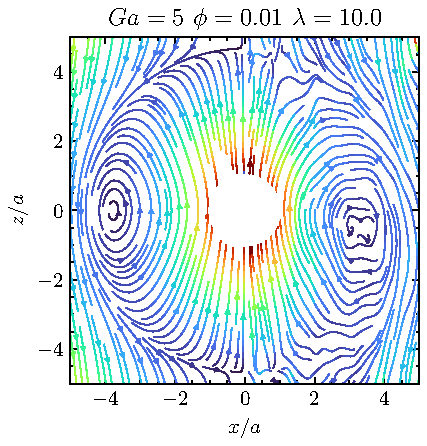
\includegraphics[width = 0.32\textwidth]{image/HOMOGENEOUS_final/Stream/Stream_PHI_1_Ga_5_l_10.pdf}
    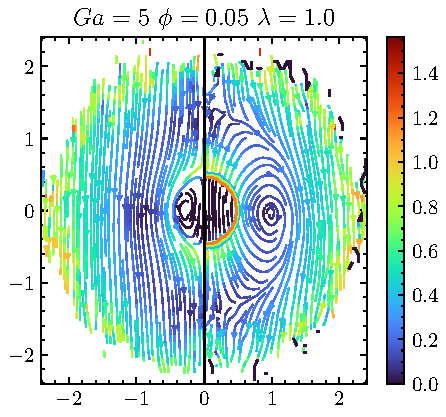
\includegraphics[width = 0.32\textwidth]{image/HOMOGENEOUS_final/Stream/Stream_PHI_5_Ga_5_l_10.pdf}
    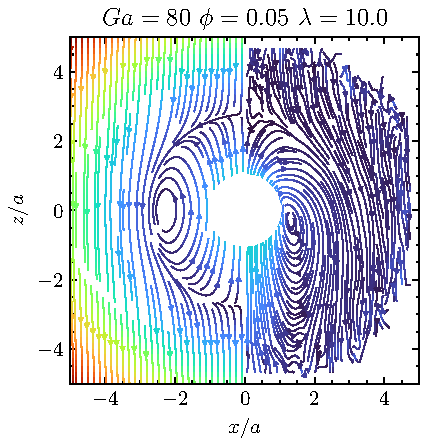
\includegraphics[width = 0.32\textwidth]{image/HOMOGENEOUS_final/Stream/Stream_PHI_5_Ga_80_l_10.pdf}
    \caption{Streamlines of the disturbance velocity field $\textbf{v}^\text{nst}$, in the cross-section given by the plane $(\textbf{e}_x,\textbf{e}_z)$, for two volume fractions $\phi = 0.01$ (left) and $\phi = 0.05$ (middle) at $\lambda = 10$ and $Ga = 5$.
    (right) plot of the inertial case $Ga = 80$. 
    On the left side of the panel ($x/a < 0$), we have re-plotted the theoretical solution provided by \ref{eq:v_nst_solution_adim}.   
    On the right side of the panel ($x/a > 0$), we have reconstructed the streamlines obtained with the DNS, using \ref{eq:vnst_DNS}. 
    The color map indicates the magnitude of the velocity, from black which corresponds to a velocity magnitude of 0, to the color at the interface of the droplet which corresponds to a magnitude of 1.}
    \label{fig:vnst_DNS}
\end{figure}
As seen on \ref{fig:vnst_DNS}:  %the common points that shear the velocity fields from the DNS to the theoretical prediction are the following: 
(1) both velocity fields exhibit approximately the same wake close to the interface of the droplet. 
That is the wake of an isolated rising vertical droplet. 
(2) For a distance large enough from the droplet center we see the downstream flow appears.
(3) The recirculation region, delimited by the null radial velocity (i.e. for the points $\textbf{r}$ following $\textbf{v}^\text{nst}\cdot \textbf{r} = 0$ with $|\textbf{r}|>a$), follows the same trends as the theoretical prediction, i.e. the radius is smaller for higher $\phi$. 
Additionally, the radii of the recirculation region have approximately the same size for both cases where $Ga = 5$. 

Regarding the differences, we can note that for the case $\phi = 0.01$, displayed on \ref{fig:vnst_DNS} (left) the wake of the particle is slightly asymmetric, while the theoretical solution is purely symmetric. 
The fore-aft symmetry of the wake of a particle as displayed in \ref{fig:vnst_vertical} is typically due to the absence of inertial effect. 
Thus, the non-fore-aft symmetry observed on the plot, \ref{fig:vnst_DNS} (left), is due to the non-negligible inertial effect present for this case. 
Indeed, as reported in \ref{tab:simulations_recall} the \textit{Reynolds} number for this case is $Re \approx 1$, implying that the inertial effects cannot be neglected. 
In opposition at $\phi = 0.05$, the numerical results exhibit a nearly fore-aft symmetric wake. 
This is consistent with the previous remark since for this case $Re < 1$. 

To extend our understanding we have also displayed on \ref{eq:vnst_DNS} (right) a high inertial case, with  $Ga = 80$. 
In this case, we see that the wake exhibits fore-aft asymmetry, which confirms that this trend comes with inertial effects. 
Additionally, we can note that the top boundary of the recirculation region is approximately at the same location as the theoretical prediction. 
However, the downstream boundary is different from the one predicted by the theoretical prediction, again that is because the fore-aft symmetry of the flow is broken.  
The symmetry of a distribution can be quantified by the ``skewness'' of the distribution. 
In the case of the continuous phase velocity distribution it is the triple velocity correlation $\avg{\chi_fk_f  \textbf{u}_f'}$ appearing in the pseudo turbulent energy equation \eqref{eq:dt_hybrid_k1}, that quantify the fore-aft symmetry.
As demonstrated, in Stokes regime $\avg{\chi_fk_f  \textbf{u}_f'} = 0$ due to the fore-after symmetry of the disturbance fields of spherical particles.  
Hence, the effect of inertia, which generates a fore-aft asymmetry in the particle's wake, will not necessarily impact the velocity variance but rather the skewness of the velocity distribution. 


To conclude, we can state that \ref{eq:v_nst_solution_adim} is well representative of the velocity field reconstructed with the DNS. 
Therefore, we can be confident regarding the accuracy of our \textit{Reynolds} stress closure at least for low \textit{Galileo} numbers. 




\subsection{Vertical velocity variance}

As discussed in the previous section, in the situation reproduced by the DNS, the velocity variance is given by \ref{eq:functional_form_avg} without the contribution of the buoyancy term (see \eqref{eq:cancelation1} and \ref{eq:cancelation2}). 
Additionally, for instance, we assert that the particle vertical velocity variance $\pavg{\textbf{u}_\alpha'\textbf{u}_\alpha'}_{zz}$ is negligible  at  $Ga =5$. 
In the next subsections, we show that this assumption is indeed confirmed by the DNS results. 
However, for the horizontal velocity variance, we will observe that it is not necessarily a valid assumption. 
Under these conditions, the vertical component of the velocity variance given by \ref{eq:functional_form_avg} is expressed as, 
\begin{equation}
    \frac{\avg{\chi_f \textbf{u}_f'\textbf{u}_f'}_{zz}}{\phi_f U^2}
    = \phi^{2/3} \left(
        \frac{2}{3}C_e^{(1)}+ C_e^{(2)}
    \right)
    = 
    \phi^{2/3}\Gamma\left(\frac{1}{3}\right) \frac{7}{60}\frac{(2+3\lambda)^2 }{(\lambda+1)^2}
    % \left(e^{-Re} - 1 \right)/2
    + \mathcal{O}(\phi), 
    % . 
    \label{eq:theoritical_simplified}
\end{equation}
where we recall that $\Gamma(1/3) \approx 2.67894$. 




\subsubsection{Comparison with the DNS}

In \ref{fig:uuyy} we compared the vertical velocity variance given by \ref{eq:theoritical_simplified} to the numerical results.
At low volume fraction and for all $\lambda$ very good agreements are obtained. 
Interestingly for all $\lambda$, \ref{eq:theoritical_simplified} seems to provide a good estimation for the Reynolds stress even at high volume fraction $\phi$, especially viscous droplets ($\lambda = 10$). 
Since no particle interaction terms of any kind are considered in the theory, this good agreement is likely coincidental.
\begin{figure}
    \centering
    % 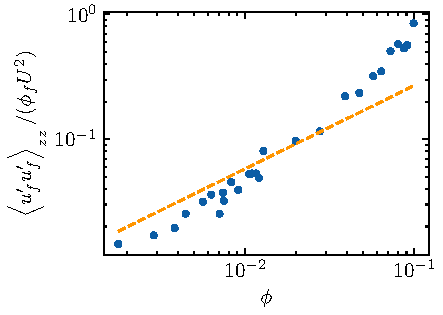
\includegraphics[height = 0.25\textwidth]{image/HOMOGENEOUS_final/CA/cartellier.pdf}
    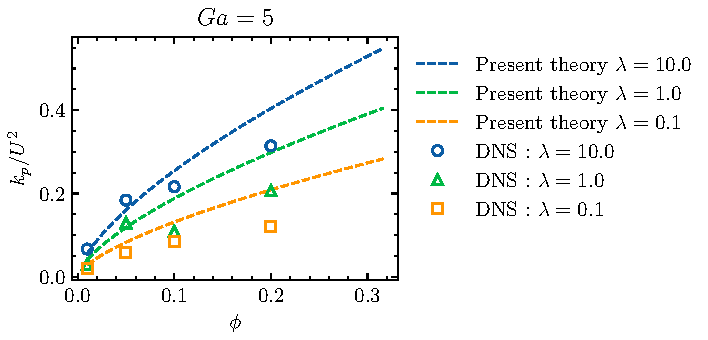
\includegraphics[height = 0.25\textwidth]{image/HOMOGENEOUS_final/CA/UUyy_Ga_5.pdf}
    \caption{Dimensionless value of the vertical velocity variance  in terms of the volume fraction $\phi$ for various $\lambda$ in the low inertial regime ($Ga = 5$). 
    % (left) Experimental  results  of \citet{cartellier2009induced} compared to \ref{eq:theoritical_simplified} with $\lambda = 0$ (dash dotted line) original scaling of \citet{cartellier2009induced}. 
    Comparison of the ``Present theory'' \eqref{eq:theoritical_simplified} against the velocity variance obtained with DNS results according to \eqref{eq:def_uuf_num}. 
    }
    \label{fig:uuyy}
\end{figure}
The red dashed line in \ref{fig:uuyy} (right) represents the potential flow solution of \citet{van1998pseudo} given by \ref{eq:van_wingarden_sol}. 
This model underpredicts the magnitude of the vertical pseudo-turbulence.
We deduce that the velocity variance produced by particles in Stokes flow is largely superior to in potential regime. 


\subsubsection{Comparison with the literature}

In \ref{fig:uuyy2}  we compare \ref{eq:theoritical_simplified} with $\lambda = 0$ to the  experimental measurements of \citet{cartellier2009induced}. 
We observe reasonable agreements from $\phi = 10^{-3}$ to moderate volume fraction ($\phi \approx 0.03$). 
In the low volume fraction regime \citet{cartellier2009induced} found that $\avg{\chi_f\textbf{u}_f'\textbf{u}_f'} / U^2 \sim \phi^{0.7 \pm 0.03}$,  while \ref{eq:theoritical_simplified} with $\lambda = 0$ predicts, $\avg{\chi_f\textbf{u}_f'\textbf{u}_f'} / U^2 \sim 1.25017 \cdot \phi^{2/3} $. 
Thus, our results overestimate \citet{cartellier2009induced} best fits by $25\%$. 
This can be explained by the non-negligible inertial effects present in \citet{cartellier2009induced} experiments, indeed they measured $Re \approx 10$ while our theory is valid in Stokes flow. 
\begin{figure}
    \centering
    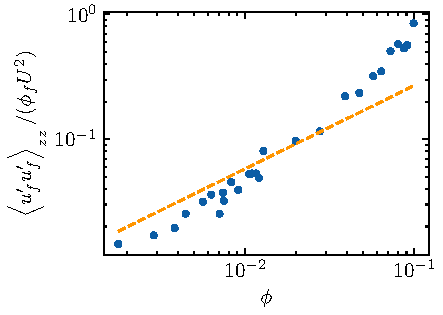
\includegraphics[height = 0.25\textwidth]{image/HOMOGENEOUS_final/CA/cartellier.pdf}
    \caption{Dimensionless value of the vertical velocity variance  in terms of the volume fraction $\phi$ for various $\lambda$ in the low inertial regime ($Ga = 5$). 
    (dots) Experimental  results  of \citet{cartellier2009induced}.
    (dashed line) Theoretical formula \ref{eq:theoritical_simplified} with $\lambda = 0$.
    (dash dotted line) \citet{cartellier2009induced}'s original scaling. 
    }
    \label{fig:uuyy2}
\end{figure}

It is reasonable to assume that the slight disparities observed between these results and the theory are due to the inertial effects or a non-negligible volume fraction effect. 
Thus, Considering the good agreements obtained with both, the numerical results and \citet{cartellier2009induced} experiments, we can state that \ref{eq:theoritical_simplified} is validated. 

\subsection{The Horizontal velocity variance}

Now that the vertical component of the velocity variance is validated, we turn our attention to the validation of the components in the normal direction to the gravity. 
Using the general formulation \ref{eq:functional_form_avg}, we write the horizontal component of the \textit{Reynolds} as, 
\begin{equation}
    \frac{\avg{\chi_f \textbf{u}_f'\textbf{u}_f'}_{xx}}{\phi_f U^2}
    = \phi^{2/3}\Gamma\left(\frac{1}{3}\right) \frac{1}{240}\frac{(2+3\lambda)^2 }{(\lambda+1)^2}
    + 
    C^{(1)}_e \left[
    \frac{\pavg{\textbf{u}_\alpha'\textbf{u}_\alpha'}_{xx}}{n_p U^2}
    - \frac{2k_p}{3U^2}  
    \right]
    + C^{(2)}_e
    \frac{2k_p}{U^2}  
    \label{eq:Horizontal_varience}
\end{equation}
Note how the first term on the right-hand side of \ref{eq:Horizontal_varience} is smaller than the one provided by \ref{eq:theoritical_simplified} ($1/240$ Vs. $7/60$). 
This means that the horizontal velocity variance produced by the mean vertical motion of the droplets is significantly lower than the vertical velocity variance. 
Additionally, in this formulation we have kept the terms related to the particle center of mass velocity variance. 


In \ref{fig:uuxx} (right) we display the numerical values of the horizontal velocity variance against the theoretical results provided by, \ref{eq:Horizontal_varience}. 
\begin{figure}
    \centering
    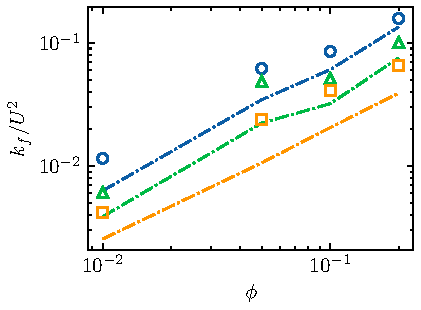
\includegraphics[height = 0.25\textwidth]{image/HOMOGENEOUS_final/CA/UUxx2_Ga_5.pdf}
    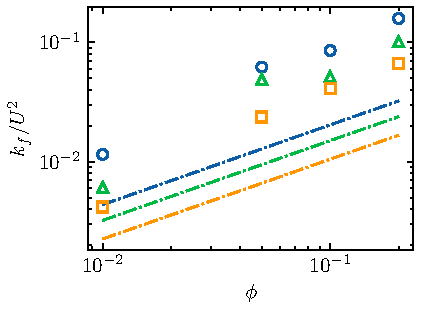
\includegraphics[height = 0.25\textwidth]{image/HOMOGENEOUS_final/CA/UUxx_Ga_5.pdf}
    \caption{Dimensionless value of the horizontal velocity varience  in terms of the volume fraction $\phi$ for various $\lambda$ in the low inertial regime ($Ga = 5$). 
    (left) Theoretical results \eqref{eq:Horizontal_varience} \underline{with} the particle velocity variance included
    (right) Theoretical results  \eqref{eq:Horizontal_varience} \underline{without} the particle velocity variance included. 
    }
    \label{fig:uuxx}
\end{figure}
It is seen that for all $\phi$ and $\lambda$ the theoretical predictions given by \ref{eq:Horizontal_varience}(right), when neglecting the particle phase velocity, i.e.  $k_p =0$ and $ \pavg{\textbf{u}_\alpha'\textbf{u}_\alpha'}_{xx} = 0 $, is underestimating the continuous phase velocity variance. 
Since the velocity variance produced by a Stokes disturbance field will be always larger (in dimensionless form) than the disturbance field given by an inertial particle, we must conclude that the lake of velocity variance predicted by the theory is due to the non-inclusion of the particle phase velocity variance. 
Indeed, according to \ref{fig:vnst_DNS} it seems that we can predict the effect of volume fraction on the averaged wake of the particle \eqref{eq:Horizontal_varience}.
Thus, the only reason why the fluid phase velocity variance is underestimated must be because of the absence of the particle phase velocity variance in this first approximation.  

On \ref{fig:uuxx} (left) we display the numerical values of the horizontal velocity variance against the theoretical results provided by, \ref{eq:Horizontal_varience}, including the values of $k_p$ and $\pavg{\textbf{u}_\alpha'\textbf{u}_\alpha'}_{xx}$ that is obtained with the DNS. 
The prediction in the dense regime ($\phi = 0.2$) seems greatly improved, while not many changes can be observed for the dilute regime. 
Indeed, in the dilute regime, we still obtain a significant error. 
At this stage it is hard to explain where does these differences come from however we can stipulate that the predicted magnitude of the velocity variance is greatly improved when including the particle phase center of mass variance. 

We can suppose that due to the relatively low magnitude of the horizontal velocity variance of the average wake of particles, the particle phase variance can no longer be neglected and must be accounted for. 
Thus, when developing an algebraic model for the \textit{Pseudo-turbulent} tensor, it is essential to consider the impact of the particle phase velocity variance, at least in the horizontal direction. 
Thus, a closure model for the particle phase velocity variance should be constructed first and incorporated into the \textit{Reynolds stress} model as outlined in \ref{eq:functional_form_avg} to remain consistent.

Nevertheless, in this chapter, we focus only on the modeling of the continuous phase velocity variance. 
We will model the particle phase velocity variance in the next chapter. 
Thus, in the subsequent sections, we make use of the particle center of mass velocity variance collected with the DNS to ensure a consistent modeling of the continuous phase \textit{Reynolds} stress.    


\subsection{Extension to higher inertial effects. }

In this subsection, we extend our model to higher \textit{Reynolds} numbers by making use of the DNS results. 
We assume the following properties to construct our semi-empirical model: 
(1) In the low inertial regime ($Re=0$) and low volume fraction ($\phi=0$) the \textit{Reynolds stress} must be given by  \ref{eq:functional_form_avg}. 
(2) The functional form given by \ref{eq:functional_form_avg} is preserved at finite $Re$ for the non-buoyancy terms. 
This means that the scalar $C_e^{(1)}$ and $C_e^{(2)}$ are the only degrees of freedom that we can use to include the finite inertial effects. 
(3) The semi-empirical expression  $C_e^{(1)}$ and $C_e^{(2)}$ should not take into account the effect of the particle phase velocity variance. 
Indeed, these are already taken into account through the terms $\pavg{\textbf{u}_\alpha'\textbf{u}_\alpha'}$ and $k_p$ in \ref{eq:functional_form_avg}. 
This means that we must perform a fit of $C_e^{(1)}$ and $C_e^{(2)}$ on the numerical data while including the particle velocity variance in \ref{eq:functional_form_avg}, that is directly obtained with the DNS.
In the subsequent chapter, we seek an analytical expression for $\pavg{\textbf{u}_\alpha'\textbf{u}_\alpha'}$ to close entirely \ref{eq:functional_form_avg} based on theoretical analysis.

In \ref{eq:functional_form_avg} the effects of inertia could be captured directly through the constant $A = Ga^2 /(12 Re)$. 
However, it has been found that this method yields no suitable results. 
This is because the formulation of $A$ is only valid in the Stokes flows. 
Indeed, \ref{eq:v_b_sol} is a singularity solution only valid in Stokes flows. 
Thus, we still consider that $C_k^{(2)}$ and $C_{ek}^{(2)}$ cancel-out according to \ref{eq:cancelation1} and \ref{eq:cancelation2} and play on the other parameters, i.e. $C_e^{(1)}$ and $C_e^{(2)}$,  to include inertial effects. 

In the following we first focus on the modeling of the trace of the \textit{Reynolds} stress, then once it is done we concentrate on the deviatoric part of this tensor. 

\subsubsection{The pseudo turbulent kinetic energy}

According to \ref{eq:functional_form_avg} the pseudo turbulent kinetic energy of the continuous phase can be written at $Re = 0$ and $\phi = 0$ by,
\begin{equation}
    k_f^{Re = 0}
    = 
    C_e^{(2)}  \left( U^2 + 2 k_p\right)  \frac{3}{2}
    % + \frac{3}{2} (C_k^{(2)} + C_{ek}^{(2)})
    \label{eq:TKE}
\end{equation}
We recall that in the stokes flow regime $C_k^{(2)}$ and $C_{ek}^{(2)}$ cancel-out. 
We propose the following semi-empirical formulation to express the fluid phase kinetic energy: 
\begin{equation}
    k_f
    = 
    k_f^{Re = 0}
    \cdot \frac{\left(e^{-Re} +1\right)}{2}.
    \label{eq:semi_empirical}
\end{equation}


In  \ref{fig:kf} we display the values of $k_f$ obtained with the DNS against the semi-empirical formula given by \ref{eq:semi_empirical} with (dot-dashed lines) and without (dashed lines) the particle phase velocity variance. 
We can observe that \ref{eq:semi_empirical} with the particle phase velocity variance included, fit reasonably all of our numerical results. 
We note that \ref{eq:semi_empirical} without $k_p$ (dashed lines) seem to underpredict the fluid phase velocity variance for $\phi = 0.2$. 
At lower volume fraction it is not clear whether it improves the predictions or not. 
Anyhow, for $\phi \le 0.1$ the particle phase velocity variance seems negligible compared to the averaged wake contribution. 

Consequently, this rather simple formula \eqref{eq:semi_empirical},  fits nicely all of our numerical results regardless of the viscosity ratio, \textit{Reynolds} numbers, and volume fraction.  
Thus, according to \ref{eq:semi_empirical}, it appears that the contribution of finite inertial effect leads to a reduction by a factor of 2 in the magnitude of the fluid phase kinetic energy when the \textit{Reynolds} number is large enough. 
Surprisingly, the dependence with $\phi$ and $\lambda$ do not seem to be affected by greater \textit{Reynolds} number, as witnessed by the absence of $\phi$ and $\lambda$ in \ref{eq:semi_empirical}. 
\begin{figure}
    \centering
    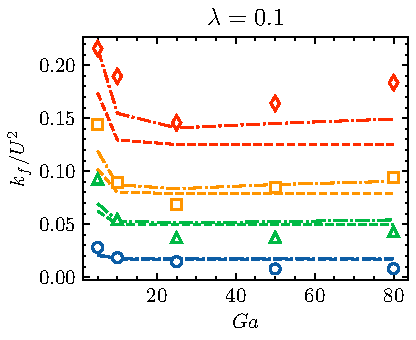
\includegraphics[height = 0.25\textwidth]{image/HOMOGENEOUS_final/CA/KF2_l_0.pdf}
    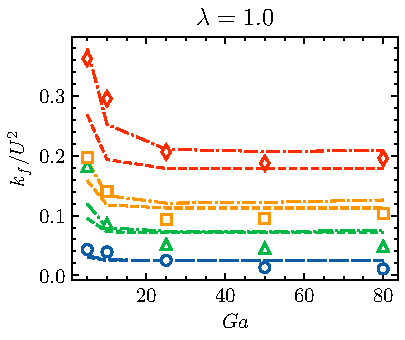
\includegraphics[height = 0.25\textwidth]{image/HOMOGENEOUS_final/CA/KF2_l_1.pdf}
    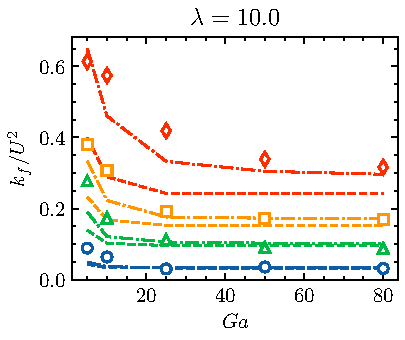
\includegraphics[height = 0.25\textwidth]{image/HOMOGENEOUS_final/CA/KF2_l_10.pdf}
    \caption{Dimensionless continuous phase pseudo turbulent energy, $k_f/U^2$ in terms of the \textit{Galileo} number.
    (left) $\lambda = 0.1$
    (middle) $\lambda = 1$
    (right) $\lambda = 10$
    (Symbols) DNS results computed according to \ref{eq:def_uuf_num}
    ($\pmb\bigcirc$) $\phi = 0.01$; ($\pmb\triangle$) $ \phi = 0.05$; ($\pmb\square$) $\phi = 0.1$ ($\pmb\lozenge$) $\phi = 0.2$.
    (dot-dashed lines) Semi-empirical formula \ref{eq:semi_empirical} \underline{including} the results of the DNS for the particle phase velocity fluctuations. 
    (dashed lines) Semi-empirical formula \ref{eq:semi_empirical} \underline{excluding} the particle phase velocity fluctuations. 
    }
    \label{fig:kf}
\end{figure}


\subsubsection{Deviatoric part of the Reynolds stress tensor}


From \ref{eq:functional_form_avg} we define the Deviatoric normalized part of the \textit{Reynolds Stress}, as, 
\begin{equation}
    \textbf{D} =
    \frac{3\avg{\chi_f\textbf{u}_f'\textbf{u}_f'}}{2 k_f} - 1
    = 
    b_f^{Re,\phi = 0} \left[
        \textbf{e}_p\textbf{e}_p
        + \frac{\pavg{\textbf{u}_\alpha'\textbf{u}_\alpha'}}{n_p U^2}
         - \frac{1}{3}(\textbf{e}_p\cdot \textbf{e}_p+2k_p/U^2)\bm\delta
    \right]
    \label{eq:D_def}
\end{equation}
Where the constant $b_f^{Re,\phi =0} = \frac{27}{10}$ in the Stokes and dilute regime \eqref{eq:constants}. 
To extend the domain of validity of \textbf{D} we must adjust the scalar $b_f^{Re,\phi = 0}$ to higher $Re$, and $\phi$.  


In \ref{fig:bf} we display the vertical (hollow symbols) and horizontal (filled symbols) components of $\textbf{D}$. 
It is shown that a good semi-empirical fit for $b_f$ is given by, 
\begin{equation}
    b_f = \frac{27}{10}  \text{exp}\left\{- 3\left(\phi^{5/6} + \frac{10^{-3}}{\lambda+1}Re\right)\right\}. 
    \label{eq:b_f}
\end{equation}
\begin{figure}
    \centering
    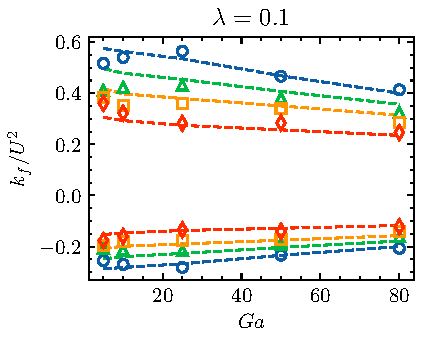
\includegraphics[height = 0.25\textwidth]{image/HOMOGENEOUS_final/CA/D2_l_0.pdf}
    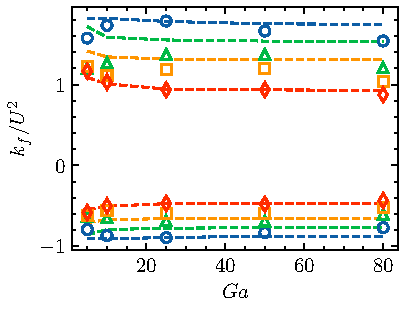
\includegraphics[height = 0.25\textwidth]{image/HOMOGENEOUS_final/CA/D2_l_1.pdf}
    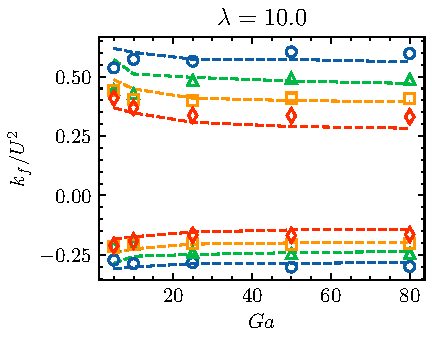
\includegraphics[height = 0.25\textwidth]{image/HOMOGENEOUS_final/CA/D2_l_10.pdf}
    \caption{Deviatoric part of the \textit{Reynolds stress} tensor, $\textbf{D}$, in terms of the \textit{Galileo} number for multiple viscosity ratios:
    (left) $\lambda = 0.1$,
    (middle) $\lambda = 1$,
    (right) $\lambda = 10$. 
    (Symbols) DNS results computed according to \ref{eq:def_uuf_num}, (hollow symbols) $\textbf{D}_{yy}$ and (filled symbols) $\textbf{D}_{xx}$. 
    (dot-dashed lines) Values of $\textbf{D}_{xx}$ given by \ref{eq:D_def} using \ref{eq:b_f}, including the particle phase velocity fluctuations obtained with the DNS. 
    (dashed lines) Values of $\textbf{D}_{yy}$ given by \ref{eq:D_def} using \ref{eq:b_f}
    ($\pmb\bigcirc$) $\phi = 0.01$; ($\pmb\triangle$) $ \phi = 0.05$; ($\pmb\square$) $\phi = 0.1$ ($\pmb\lozenge$) $\phi = 0.2$.
    }
    \label{fig:bf}
\end{figure}
We clearly observe that $b_f/b_f^{Re,\phi = 0}$ varies with $\phi$, $\lambda$ and the $Re$, while $k_f/k_f^{Re = 0}$ where just a function of $Re$. 
Specifically, for $\lambda = 10$ we observe that $b_f$ depends weakly on $Re$ or $Ga$, where it is a lot more dependent for bubbles. 

% This may be in contradiction with the results of \citet{mehrabadi2015pseudo} as his fitted constant $b_f$ is $Re$ dependent for solid sphere, i.e. $\lambda = \infty$. 
% Indeed, they $b_f$ reads in our notation as, 
% \begin{equation*}
%     \frac{0.523}{1+0.305 e^{-0.114}} \text{Exp}\left\{\frac{-3.511}{1+1.801 e^{-0.005Re(1-\phi)}}\right\}
% \end{equation*}
% This dispersencies in the results is still unclear to us.  


Although \ref{eq:b_f} and \ref{eq:semi_empirical} do not match exactly the numerical results, we prefer not to overfit our results and kept a rather simple fit for $b_f$ and $k_f$. 
In summary, with the constant $b_f$ and $k_f$ fitted on our numerical results we extended our \textit{Reynolds stress} model for higher $Re$, $\phi$, and $\lambda$. 
It must be remembered that since we studied only vertically rising buoyant bubbly flow we only extended the validity of this fit in this specific configuration. 



\subsection{Final validation}

We would like to end this section with a series of validations comparing our final model to the experimental and numerical results at finite \textit{Reynolds number}. 

On \ref{fig:trygvason} we first display the pseudoturbulence kinetic energy Vs. a series of numerical results from \citet{bunner2002dynamics,loisy2016direct,wang2021numerical} and experimental results of \citet{martinez2007measurement}.  
We can observe that the predicted magnitude of $k_f$ is in very good agreement with all these results. 
These studies concern either fixed arrays of particles or dilute suspensions of particles, in both cases the particle velocity variance is negligible, thus we consider that $k_p = 0$ in \ref{eq:semi_empirical}. 
We can observe that setting $\lambda \to\infty$ in \ref{eq:semi_empirical}, captures quantitatively the results of \citet{wang2021numerical} for solid particle fixed array. 
It also seems to correspond to the pseudo turbulence generated by the experimental results of \citet{martinez2007measurement} which considered rising bubbles in water. 
We assume that, because their bubbles are contaminated this can be considered as a no-slip boundary condition at the surface of the bubbles, which hence correspond to solid particles, i.e. $\lambda \to \infty$.  
\begin{figure}
    \centering
    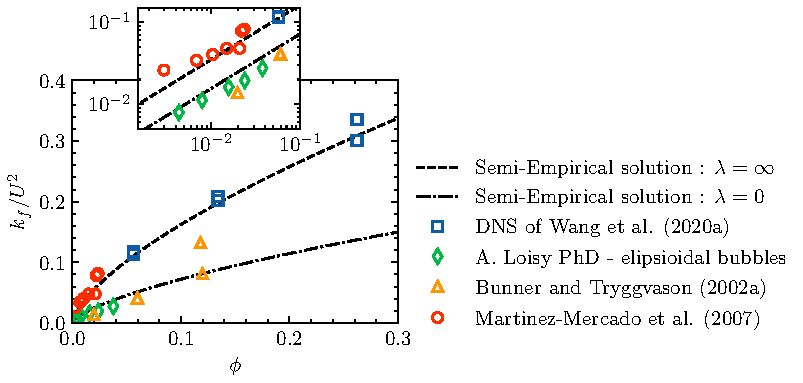
\includegraphics[height = 0.35\textwidth]{image/HOMOGENEOUS_final/CA/KFliterature.pdf}
    \caption{Dimensionless continuous phase pseudo turbulent energy, $k_f/U^2$ in terms of the \textit{Galileo} number.
    (Symbols) DNS and experimental results of: 
    ($\pmb\square$)  Particle-resolved Direct Numerical Simulations (PR-DNS)
    of fixed solid spherical particle assemblies at $20< Re < 100$  by \citet{wang2021numerical}; 
    ($\pmb\lozenge$) Direct numerical simulation (DNS) of rising deformable bubbles at $Re \approx 30$ \citep{loisy2016direct}
    ($\pmb\triangle$) DNS of rising spherical bubbles by \citet{bunner2002dynamics}. 
    ($\pmb\bigcirc$) Experiment of rising spherical bubbles in water by \citet{martinez2007measurement} at $Re \approx 30$. 
    (dot-dashed lines) Semi-empirical formula \ref{eq:semi_empirical} at $Re \approx 30$ with $\lambda = 0$. 
    (dashed lines)  Semi-empirical formula \ref{eq:semi_empirical} at $Re \approx 30$ with $\lambda = \infty$.
    }
    \label{fig:trygvason}
\end{figure}
In \ref{fig:trygvason} we also compared our analytical formula to the DNS results of \citet{bunner2002dynamics} and \citet{loisy2016direct} which considered rising bubbly flows. 
As can be seen from the (dashed lines) in \ref{fig:trygvason} our semi-empirical formula captures quantitatively their results. 

As the previous validation concerned the low but finite \textit{Reynolds number} regime, we now challenge ourselves and compare our semi-empirical formula \eqref{eq:semi_empirical} to DNS out of our range of \textit{Reynolds} numbers. 
In \citet{mehrabadi2015pseudo} they performed DNS of a fixed array of spherical solid spheres, from $Re_m = 1$ to $Re_m=300$ where $Re_m = (1- \phi) Re$ is the Reynolds number based on the mean slip velocity. 
\begin{figure}
    \centering
    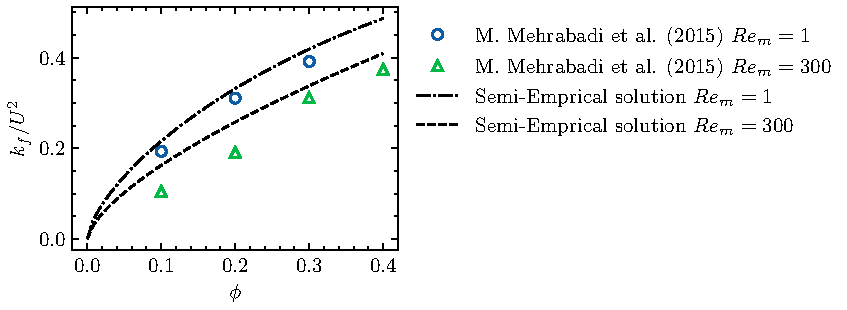
\includegraphics[height = 0.25\textwidth]{image/HOMOGENEOUS_final/CA/tenneti.pdf}
    \caption{Dimensionless continuous phase pseudo turbulent energy, $k_f/U^2$ in terms of the volume fraction $\phi$.
    (Symbols) 
    results of Particle-resolved Direct Numerical Simulations
    of fixed particle assemblies by \citet{mehrabadi2015pseudo}
    ($\pmb\bigcirc$) $Re_m = (1-\phi) \approx 1$; ($\pmb\triangle$) $Re_m \approx 300$;
    (dot-dashed lines) Semi-empirical formula \ref{eq:semi_empirical} at $Re_m = 1$
    (dashed lines) Semi-empirical formula \ref{eq:semi_empirical} at $Re_m = 300$
    }
    \label{fig:tennet}
\end{figure}
As shown in \ref{fig:tennet} (dot-dashed line), the results at low Reynolds number ($Re_m=1$) of \citet{mehrabadi2015pseudo}  correspond quantitatively to \eqref{eq:semi_empirical}. 
However, we can remark that at $Re_m = 300$, the relation $k_f \sim \phi^{2/3}$, seems not valid anymore, even at low $\phi$. 
This is evidenced by the empirical formula proposed by \citet{mehrabadi2015pseudo}, see Eq (7.1) of their paper. 
Nevertheless, it is remarkable that \ref{eq:semi_empirical} still provides a reasonable quantitative prediction, even at $Re_m = 300$. 


Finally, to validate the functional form of \ref{eq:functional_form_avg} regarding the inclusion of the particle phase velocity variance, we compare our results to the study of \citet{shajahan2023inertial}. 
They performed DNS of free arrays of solid particles under sedimentation.  
\begin{figure}
    \centering
    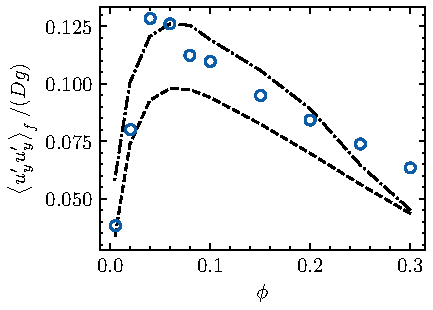
\includegraphics[height = 0.25\textwidth]{image/HOMOGENEOUS_final/CA/tariq.pdf}
    \caption{Dimensionless vertical velocity varience, in terms of the volume fraction $\phi$. 
    (Symbols) results of Particle-resolved Direct Numerical Simulations  of gravitational settling of monodisperse solid spheres by \citet{shajahan2023inertial} at $Ga = 144$. 
    (dot-dashed lines) Semi-empirical formula \underline{including} \citet{shajahan2023inertial}'s results for the particle phase velocity fluctuations. 
    (dashed lines) Semi-empirical formula \underline{excluding} the particle phase velocity fluctuations. 
    }
    \label{fig:tariq}
\end{figure}
We can observe on \ref{fig:tariq} (dashed lines) that the semi-emprical formula slightly underestimates the result when we neglect the particle phase velocity variance. 
When we include the contribution of the particle phase velocity variance (that we obtained in their study), we can note that the prediction improved a lot. 
We conclude that the general functional form of \ref{eq:functional_form_avg} seems to capture the dependence of the \textit{Reynolds} stress with the particle phase velocity variance. 
